\section{Introduction}
\label{sec:intro}

Reconstructing and editing 3D scenes from multi-view images is an important task in computer graphics and computer vision. 
Recently, Neural Radiance Fields \yl{(NeRFs)}~\cite{NeRF} have shown promising results in novel view synthesis, based on which a number of editing methods~\cite{NeuMesh, NeuTex, EditNeRF, DE-NeRF} are proposed. 
However, NeRF-based methods require dense sampling of camera rays, making rendering less efficient. 
Gaussian splatting~\cite{GS} instead approximates a scene with a set of \yl{3D Gaussians} and visualizes it with a rasterization-based renderer to achieve real-time performance. 
However, despite high-quality and efficient rendering, \yl{Gaussian} splatting still lacks the ability of editing. 


In the original \yl{Gaussian} splatting representation, the appearance is approximated by a view-related spherical harmonic function which entangles both texture and lighting information, \yl{making} separate texture and lighting editing impossible. 
\wt{Independent editing requires texture and lighting decomposition so that one part can be manipulated without influencing the other. 
However, different from 3D representations like textured \yl{meshes} or \yl{NeRFs} that have an explicit surface or a continuous implicit field, which can provide a good geometry basis like normal direction for the texture and lighting decomposition, \yl{Gaussian} splatting models a scene's geometry with a discrete set of \yl{Gaussians}, and \yl{this} discrete representation makes the geometry less tractable, posing challenges for later texture and lighting decoupling.} 




\begin{figure}[t!]
  	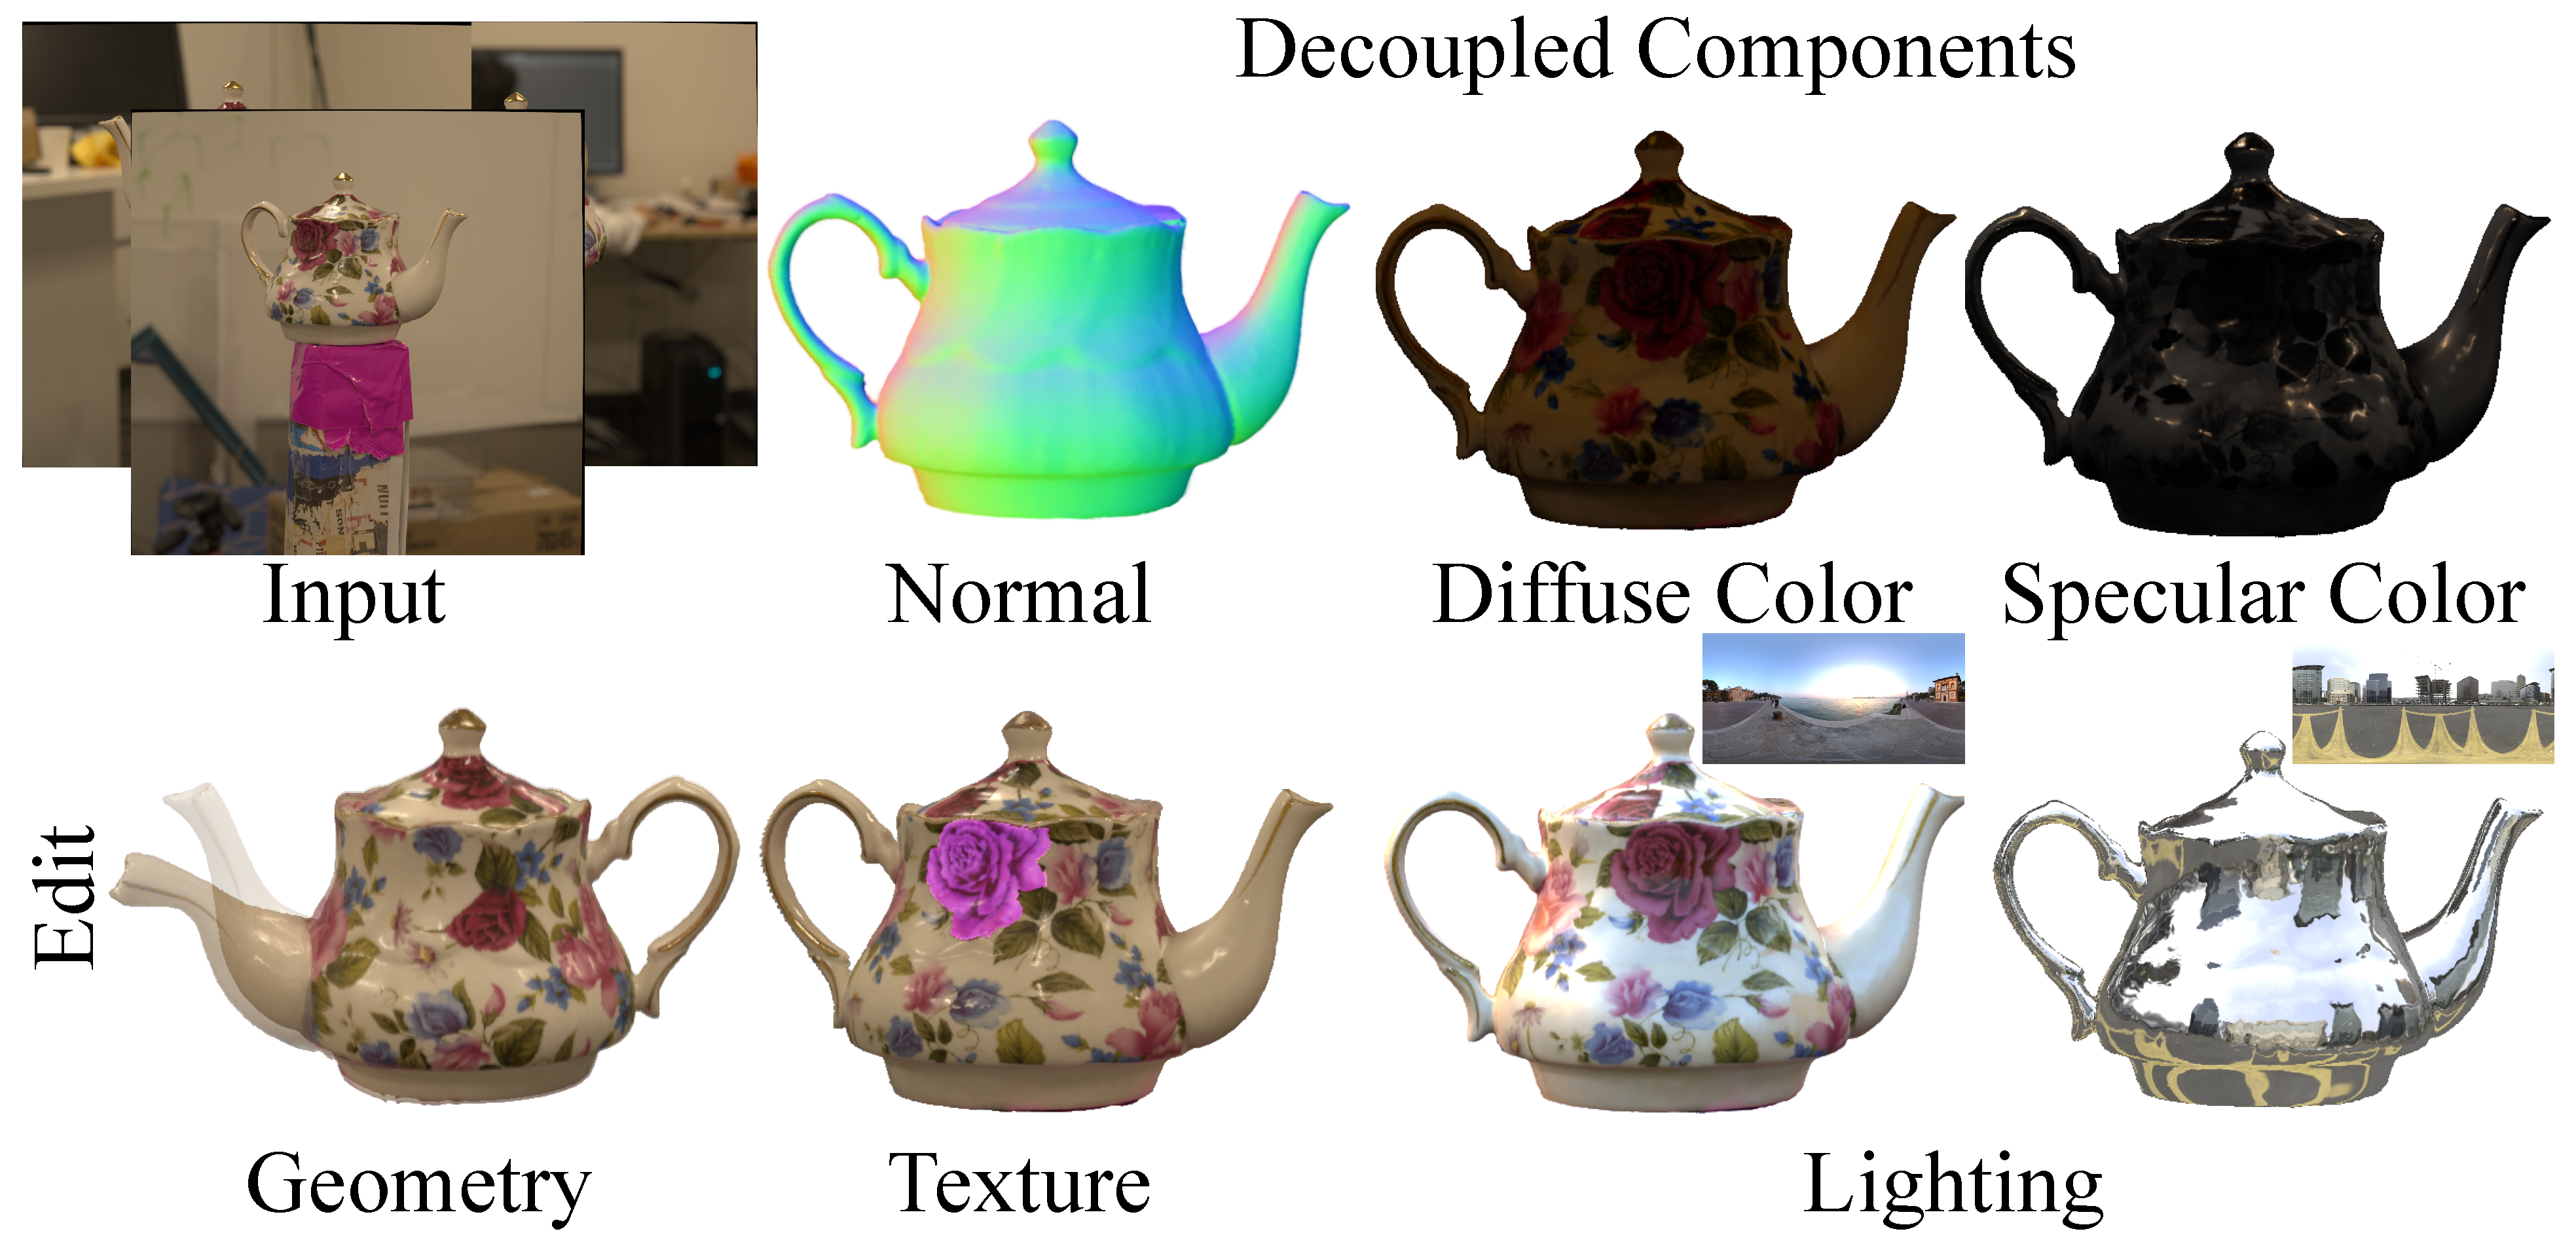
\includegraphics[width=0.99\linewidth]{./img/teaser_teapot_scene001}
    \vspace{-1mm}
    \caption{
        Given multi-view images, \name optimizes a \yl{Gaussian} splatting representation with decoupled geometry, texture, and lighting. 
        With this decoupled representation, \name not only allows geometry and texture editing, but \yl{can also} render the input scene (the 3rd column, bottom row) or the edited scene (the last column, bottom row) under a novel illumination. 
    }
    \vspace{-5mm}
    \label{fig:teaser}
\end{figure}






Recently, in the context of \yl{Gaussian} splatting, a few methods have made attempts to edit it. 
\yl{Two independent works both named}
GaussianEditor~\cite{GaussianEditor,GaussianEditor_text} utilize the 2D segmentation model~\cite{SAM} and text-to-image diffusion models~\cite{Diffusion} to enable scene editing like object removal/insertion or text-guided modification similar to Instruct-NeRF2NeRF~\cite{Instruct-NeRF2NeRF}. 
To enable better-controlled editing on texture and lighting, \yl{the works}~\cite{RelightableGaussian, GS-IR, GaussianShader, GIR} try to disentangle texture and lighting to enable individual editing for both diffuse scenes and reflective scenes. 
Although obtaining plausible decomposition results, they use \textit{forward shading} that first calculates shading for each \yl{Gaussian} and then blends shaded \yl{Gaussians}, which can cause blending artifacts when %
the scene is relighted.
This is because the geometry attributes of \yl{Gaussians} like opacity are optimized under the input lighting condition while under novel illuminations shaded \yl{Gaussians} might be blended in a wrong way (\yl{see} 3rd to 6th 
 rows in Fig.~\ref{fig:relight} \yl{for some examples}). 
In addition, they \yl{learn} geometry from the \yl{Gaussian} splatting representation with the normal direction derived from \yl{the} rendered depth map so their geometry may contain \yl{noise} and degenerate on scenes with reflective surfaces (\yl{see} the ``Normal" rows in Fig.~\ref{fig:decom}). 

To resolve the aforementioned issues, we propose \name that decouples a scene's texture and its surrounding illumination of the \yl{Gaussian} splatting representation with \yl{the} \textit{deferred shading} technique. 
Given multi-view captures of an input scene, we define a set of \yl{Gaussians} with extra learnable texture attributes and normal directions attached to model texture and geometry respectively. 
To enable faithful geometry reconstruction, we distill the normal field from a signed distance function \yl{(SDF)} onto the \yl{Gaussians}. 
We also optimize a learnable environment map to approximate the surrounding lighting conditions. 
In the rendering process, geometry and texture buffers are first rasterized and shading is calculated at the pixel level with the \textit{deferred shading} technique to enable faithful decoupling and editing. 
\wt{Despite involving more complex shading computation, \name still allows real-time rendering ($\sim$30FPS at $800 \times 800$ resolution on a single 3090 GPU).}

Our contributions are as follows:
\begin{itemize}
    \item We introduce \name, a decoupled \yl{Gaussian} splatting representation with editable geometry, texture and lighting, where its geometry is enhanced by a normal distillation module. 
    \item \yl{To the best of our knowledge,} \name is the first to apply the \textit{deferred shading} technique to \yl{Gaussian} splatting, which alleviates blending artifacts of previous methods.
    \item Experiments show that \yl{our} \name produces more faithful decomposition and editing results compared to previous methods. 
\end{itemize}
